% Our packages
%\usepackage{float}
%\usepackage[font=small]{caption}
%\usepackage{color}
%\usepackage{graphicx}
%\usepackage{booktabs}
%\usepackage{subcaption}
%\usepackage{hyperref}
%\usepackage[utf8]{inputenc}
%\usepackage{tabularx}
%\usepackage{tablefootnote}
%\usepackage{amsmath}
%\usepackage{amssymb}
%\usepackage{placeins}
%\usepackage{scrextend}

%\title{Tell Me Why: Using Question Answering as Distant Supervision for Answer Justification}


%\begin{abstract}
%
%For many applications of question answering (QA), being able to explain why a given model chose an answer is critical.  However, the lack of labeled data for  answer justifications makes learning this difficult and expensive.  Here we propose an approach that uses answer ranking as distant supervision for learning how to select informative justifications. 
%We propose a neural network architecture for QA that reranks answer justifications as an intermediate (and human-interpretable) step in answer selection. Our approach is informed by a set of features designed to combine both learned representations and explicit features to capture the connection between questions, answers, and answer justifications.
% We show that with this end-to-end approach we are able to significantly improve upon a strong IR baseline in both justification ranking (+9\% rated highly relevant) and answer selection (+6\% P@1).  %We also provide an error analysis that demonstrates that we can use the justifications returned to better understand what our model has learned.
%\end{abstract}

\chapter{Robust and interpretable: A neural approach  \label{chapter:emnlp2017}}

%\section{Introduction}
\label{sec-emnlp2017:intro}
%
%Developing interpretable machine learning (ML) models, that is, models where a human user can \emph{understand} what the model is learning, is considered by many to be crucial for ensuring usability and accelerating progress \cite{craven1996extracting,Kim2015MindTG, letham2015interpretable, Ribeiro2016WhySI}.  
%% bs: removed for space, we talk more about this in related work
%%As such, it has received much attention in recent years, especially as deep learning and complex architectures have seen dramatic gains in many tasks.
%For many applications of question answering (QA), i.e., finding short answers to natural language questions, simply providing an answer is not sufficient. A complete approach must be interpretable, i.e., able to {\em explain} why an answer is correct. 
%For example, in the medical domain, a QA approach that answers treatment questions would not be trusted if the treatment recommendation is not explained in terms that can be understood by the human user. 
%
%
%One approach to interpreting complex models is to make use of human-interpretable information % metric % ms: not a metric...
% generated by the model to gain insight into what the model is learning.  This can be an intermediate representation used by the model, as with the model-generated text spans of \citet{Lei2016RationalizingNP}, that serve as input to another classification network.  
%By learning these intermediate representations end-to-end with a downstream task, they are optimized to correlate with what the model learns is discriminatory for the task, and they can be evaluated against what a human would consider to be important.
%\todo{need to define what a downstream task means to use this term}, they are optimized to correlate with what the model learns is discriminatory for the task, and they can be evaluated against what a human would consider to be important.
%Here we apply this general framework for model interpretability to QA.
%
%
%\begin{table}[t]
%\begin{center}
%\begin{footnotesize}
%\begin{tabularx}{\linewidth}{p{0.13cm}p{6.8cm}}
%\multicolumn{2}{p{8cm}}{\textbf{Question:} Which of these is a response to an internal stimulus?} \\
% (A) & A sunflower turns to face the rising sun. \\
% (B) & A cucumber tendril wraps around a wire. \\
% (C) &  A pine tree knocked sideways in a landslide grows upward in a bend. \\
% (\textbf{D}) &\textbf{Guard cells of a tomato plant leaf close when there is little water in the roots .} \\
%\\
%\multicolumn{2}{p{7.2cm}}{\textbf{Justification:} 
%Plants rely on hormones to send signals within the plant in order to respond to internal stimuli such as a lack of water or nutrients. } \\
%
%\end{tabularx}
%\end{footnotesize}
%\caption{{  Example of an 8th grade science question with a justification for the correct answer.  Note the lack of direct lexical overlap present between the justification and the correct answer, demonstrating the difficulty of the task of finding justifications using traditional distant supervision methods. }}
%%space{-6mm} 
%\label{tab:question_example}
%\end{center}
%\end{table}
%
%In this work, we focus on answering multiple-choice science exam questions (Clark \citeyear{clark:2015}; see example in Table~\ref{tab:question_example}). 
%This domain is challenging as: (a) approximately 70\% of science exam question shave been shown to require complex forms of inference to solve \cite{clark:2013,jansen-EtAl:2016:COLING}, and (b) there are few structured knowledge bases to support this inference.  
%Within this domain, we propose an approach that learns to both select and explain answers, when the only supervision available is for which answer is correct (but not how to explain it).
%Intuitively, our approach chooses the justifications that provide the most help towards ranking the correct answers higher than incorrect ones.
%More formally, our neural network approach alternates between using the current model with max-pooling to choose the highest scoring justifications for correct answers, and optimizing the answer ranking model given these justifications. 
%Crucially, these reranked texts serve as our human-readable answer justifications, and by examining them, we gain insight into what the model learned was useful for the QA task.   


The specific contributions of this work are:
\begin{enumerate}
\item We propose an end-to-end neural method for learning to answer questions and select a high-quality justification for those answers. 
Our approach re-ranks free-text answer justifications without the need for structured knowledge bases. 
With supervision only for the correct answers, we learn this re-ranking through a form of distant supervision -- i.e., the answer ranking supervises the justification re-ranking. 

\item We investigate two distinct categories of features in this ``little data'' domain: explicit features, and learned representations. We show that, with limited training, explicit features perform far better despite their simplicity. 

\item We demonstrate a large (+9\%) improvement in generating high-quality justifications over a strong information retrieval (IR) baseline, while maintaining near state-of-the-art performance on the multiple-choice science-exam QA task, demonstrating the success of the end-to-end strategy.
\end{enumerate}

%\section{Related work}

In many ways, deep learning has become the canonical example of the "black box" of machine learning and many of the approaches to explaining it can be loosely categorized into two types: approaches that try to interpret the parameters themselves (e.g., with visualizations and heat maps \citep{Zeiler2014VisualizingAU,nips15_hermann, Li2016VisualizingAU}, and approaches that generate a human-interpretable metric that is ideally correlated with what is being learned inside the model (e.g., \citet{Lei2016RationalizingNP}). Our approach falls into the latter type -- 
we use our model's reranking of human-readable justifications to give us insight into what the model considers informative for answering questions.  This allows us to see where we do well (Section \ref{sec-emnlp2017:justification_results}), and where we can improve (Section  \ref{sec-emnlp2017:erroranalysis}).

Deep learning has been successfully applied to many recent QA approaches and related tasks \cite[][inter alia]{Bordes2015LargescaleSQ,nips15_hermann, He2016CharacterLevelQA, dong2015question, Tan2016ImprovedRL}.
%are enticing, and for good reason -- many recent approaches to question answering and related tasks have had much success with various deep learning models \cite[][inter alia]{Bordes2015LargescaleSQ,nips15_hermann, He2016CharacterLevelQA, dong2015question, Tan2016ImprovedRL}.  
However, large quantities of data are needed to train the millions of parameters often contained in these models.  
%Of potentially greater utility in low-data domains, 
Recently, simpler model architectures have been proposed that greatly reduce the number of parameters while maintaining high performance \cite[e.g.,][]{Iyyer2015,chen2016thorough,Parikh2016ADA}.  
%For example, \citet{Iyyer2015}'s show that with their Deep Averaged Network, which replaces complex recurrent neural networks with an average of embeddings and a few, albeit large, dense layers, they improved performance on both a sentiment analysis and a QA task.  For natural language inference, \citet{Parikh2016ADA} used a simpler neural alignment  approach with an attention mechanisms to greatly reduce the size of their model while reaching then state-of-the-art performance.  
We take inspiration from this trend and propose a simple neural architecture for our task to offset the limited available training data. 

Another way to mitigate sparse training data is to include higher-level explicit features.  Like \citet{sachan2016science}, we make use of explicit features alongside features from distributed representations to capture connections between questions, answers, and supporting text.  However, we use a simpler set of features and while they use structured and semi-structured knowledge bases, we use only free-text.  %Additionally, though we also learn to select support from our knowledge base (in some ways similar to \citeauthor{sachan2016science}'s latent answer-entailing structure), since we are explicitly trying to perform \emph{explainable} question answering, here we evaluate the justifications learned by our approach and show that they are significantly better than a  strong IR baseline (Section \ref{sec-emnlp2017:justification_results}).   

Our approach to learning justification reranking end-to-end with answer selection is similar to the \citet{jansen2017framing} latent reranking perceptron,  which also operates over free text.  However, our approach does not require decomposing the text into an intermediate representation, allowing our technique to more easily extend to larger textual knowledge bases.  
%ir approach is able to aggregate information from a variety of sources into one justification, our light-weight approach however, does not rely on a large set of heuristics and heavy pre-processing to transform free-text into a structured knowledge base.  

The way we have formulated our justification selection (as a re-ranking of knowledge base sentences) is related to, but distinct from the task of answer sentence selection \cite[][inter alia]{Wang2010ProbabilisticTM, Severyn:12,Severyn:13a,Severyn:13b,Severyn2015LearningTR,wang2015long}.  Answer sentence selection is typically framed as a fully or semi-supervised task for factoid questions, where a correctly selected sentence fully contains the answer text.
%and the problem is designed such that a correctly selected sentence will fully contain the answer text.
Here, we have a variety of questions, many of which are non-factoid.  Additionally, we have no direct supervision for our justification selection (i.e., no labels as to which sentences are good justifications for our answers), motivating our distant supervision approach where the performance on our QA task serves as supervision for selecting good justifications.  Further, we are not actually looking for sentences that \emph{contain} the answer choice, as with answer sentence selection, but rather sentences which close the "lexical chasm" \cite{Berger:00} between question and answer (demonstrated in the example in Table \ref{tab:question_example}). 


%Related work: QA, multiple choice, kaggle challenge, explanation-centered inference, model-specific work (NNs, etc)

%Latest QA papers (latest trends, attn, etc)
%Inspired by this literature (cite DAN \& SNLI, simpler better), but we add this latent layer they don’t have (justification quality). For simple archs: see Danqi Chen at ACL 2016 (similar to DAN but for reading comprehension). 

%Attention models (ACL 2016). Simple especially when you don’t have enough data.

%(visualizations vs analysis of embeddings VS correlated metric EMNLP paper, etc -- interpreting wts if DL is impossible, rather, find correlations betw those and explanatory natural language)

 
%\todo{Add a paragraph comparing against the task of answer sentence selection (see that reviewer from CL, and all those kernel-based papers by Moschitti). The difference is that in our case the answer and its justification arrive from different sources (i.e., the answer is provided in the multiple-choice exam, whereas the justification is extracted from study guides), whereas in previous answer sentence selection work the answer is included in the sentence. In our case we have to deal with bigger ``lexical chasm'' between question/answer/justification.}

%\todo{Discriminative information retrieval for question answering sentence selection(Chen and Van-Durme): Presented a method that selects sentences which contain potential answers for questions from a very large corpus (10\^7 sentences, requiring several thousand questions for training). Their results are dramatically better than Lucene across two datasets and several evaluation measures.}
%(Yih et al.,2013; Wang and Manning, 2010; Heilman and Smith, 2010; Yao et al., 2013a) and recently using neural networks (Yu et al., 2014; Severyn and Moschitti,2015; Wang and Nyberg, 2015; Yin et al.,2016)

%Answer sentence selection diff because we don't need (or want?) complete answer inclusion.

%Our sentences being selected are unlabeled.

%TAG paper!!! 
%\section{Neural justification reranking}
%\label{sec-emnlp2017:intro}

Once again, we are concerned with developing interpretable models for question answering.  In Chapter \ref{chapter:cl2017} we proposed a method for question answering that created and ranked human-readable answer justifications using performance on the QA task as the only form of supervision.  We demonstrated that not only did it outperform a strong information retrieval baseline in terms of correctly answering questions, but it also produced a higher percentage of good justifications, as rated by human annotators. The main drawback to the system was simply in the somewhat heavy cost of the sentence processing.  While this processing was able to be done offline (and so only once), the time and size burden still prevents its practical use over extremely large corpora. 

Here, we propose an approach that once again uses answer ranking as distant supervision for learning how to select informative justifications.  As with the previous approach, our justifications serve as inferential connections between the question and the correct answer while often containing little lexical overlap with either.  However, here in this  modified approach we use a  shallower representation of knowledge base sentences and we do not perform aggregation, facilitating usage over much larger resources.  
We additionally extend the linear learning framework used in Chapter \ref{chapter:cl2017} through the use of deep learning (specifically, a non-linear feed-forward neural network), as described in Section \ref{sec-emnlp2017:approach}.  
In making these modifications to increase the robustness of the approach, we purposefully maintain our interpretability -- we continue to rank and return human-readable answer justifications for our model's chosen answers.

\section{Chapter Outline}
The remainder of the chapter is organized as follows.  First, we review related work in Section \ref{sec-emnlp2017:relatedwork}.  In Section \ref{sec-emnlp2017:approach} we describe our overall neural approach for QA that reranks answer justifications as an intermediate (and human-interpretable) step in answer selection. In Section \ref{sec-emnlp2017:pipeline} we describe our neural network in more detail.  In that same section, we also describe our set of features designed to combine both learned representations (i.e. embeddings) and explicit features to capture the connection between questions, answers, and answer justifications.  Then, in Section \ref{sec-emnlp2017:experiments} we provide the details of our experimental setup and in Section \ref{sec-emnlp2017:results} we provide our reseults -- with this end-to-end approach we are able to significantly improve upon a strong IR baseline in both justification ranking (+9\% rated highly relevant) and answer selection (+6\% P@1).  In Section \ref{sec-emnlp2017:erroranalysis} we utilize our model-returned justifications in an error analysis.  Finally, in Section \ref{sec-emnlp2017:conclusions} are our conclusions.



\section{Related Work}
\label{sec-emnlp2017:relatedwork}
In many ways, deep learning has become the canonical example of the "black box" of machine learning and many of the approaches to explaining it can be loosely categorized into two types: approaches that try to interpret the parameters themselves (e.g., with visualizations and heat maps \citep{Zeiler2014VisualizingAU,nips15_hermann, Li2016VisualizingAU}, and approaches that generate human-interpretable information that is ideally correlated with what is being learned inside the model (e.g., \citet{Lei2016RationalizingNP}). Our approach falls into the latter type -- 
we use our model's reranking of human-readable justifications to give us insight into what the model considers informative for answering questions.  This allows us to see where we do well (Section \ref{sec-emnlp2017:justification_results}), and where we can improve (Section  \ref{sec-emnlp2017:erroranalysis}).

Deep learning has been successfully applied to many recent QA approaches and related tasks \citep[][inter alia]{Bordes2015LargescaleSQ,nips15_hermann, He2016CharacterLevelQA, dong2015question, Tan2016ImprovedRL}.
However, large quantities of data are needed to train the millions of parameters often contained in these models.  
Recently, simpler model architectures have been proposed that greatly reduce the number of parameters while maintaining high performance \cite[e.g.,][]{Iyyer2015,chen2016thorough,Parikh2016ADA}.  
%For example, \citet{Iyyer2015}'s show that with their Deep Averaged Network, which replaces complex recurrent neural networks with an average of embeddings and a few, albeit large, dense layers, they improved performance on both a sentiment analysis and a QA task.  For natural language inference, \citet{Parikh2016ADA} used a simpler neural alignment approach with an attention mechanism to greatly reduce the size of their model while reaching then state-of-the-art performance.  
We take inspiration from this trend and propose a simple neural architecture for our task to offset the limited available training data. 


Another way to mitigate sparse training data is to include higher-level explicit features.  Like \citet{sachan2016science}, we make use of explicit features alongside features from distributed representations (see Section \ref{sec-emnlp2017:features}) to capture connections between questions, answers, and supporting text.  However, we use a simpler set of features and while they use structured and semi-structured knowledge bases, we use only free-text.  %Additionally, though we also learn to select support from our knowledge base (in some ways similar to \citeauthor{sachan2016science}'s latent answer-entailing structure), since we are explicitly trying to perform \emph{explainable} question answering, here we evaluate the justifications learned by our approach and show that they are significantly better than a  strong IR baseline (Section \ref{sec:justification_results}).   

%Our approach to learning justification reranking end-to-end with answer selection is similar to the \citet[][described in Chapter \ref{chapter:cl2017}]{jansen2017framing} latent reranking perceptron,  which also operates over free text.  However, our approach does not require decomposing the text into an intermediate representation, allowing our technique to more easily extend to larger textual knowledge bases.  


%\todo{Discriminative information retrieval for question answering sentence selection(Chen and Van-Durme): Presented a method that selects sentences which contain potential answers for questions from a very large corpus (10\^7 sentences, requiring several thousand questions for training). Their results are dramatically better than Lucene across two datasets and several evaluation measures.}
%(Yih et al.,2013; Wang and Manning, 2010; Heilman and Smith, 2010; Yao et al., 2013a) and recently using neural networks (Yu et al., 2014; Severyn and Moschitti,2015; Wang and Nyberg, 2015; Yin et al.,2016)


\begin{figure}[t]
\begin{center}
\includegraphics[width=0.5\textwidth]{mainmatter/emnlp2017-qaj/arch_overall.png}
\caption{ Architecture of our question answering approach.  
Given a question, candidate answer, and a free-text knowledge base as inputs, we generate a pool of candidate justifications, from which we extract feature vectors.  We use a neural network to score each and then retain \textit{only} the highest-scoring justification from the pool of candidates (i.e., max-pooling), thus selecting the current best justification. This justification score serves as the score for the candidate answer itself.  The red border indicates the components that are trained online. }
\label{fig:arch_overall}
%space{-5mm}
\end{center}
\end{figure}

\section{Approach}
\label{sec-emnlp2017:approach}
One of the primary difficulties with the explainable QA task addressed here is that, while we have supervision for the correct answer, we do not have annotated answer justifications.  
Here we tackle this challenge by using the QA task performance as supervision for the justification reranking, allowing us to 
%extending a neural QA model to jointly learn both how to 
%jointly 
learn to choose both the correct answer and a compelling, human-readable justification for that answer.

Additionally, similar to the strategy \citet{chen2014fast} applied to parsing, we combine representation-based features with explicit features that capture additional information that is difficult to model through embeddings, especially with limited training data.


% ms: avoid "system" too engineering-y
The architecture of our approach is summarized in Figure \ref{fig:arch_overall}.  
Given a question and a candidate answer, we first query an textual knowledge base (KB) to retrieve a pool of potential justifications for that answer candidate.  
For each justification, we extract a set of features designed to model the relations between questions, answers, and answer justifications based on word embeddings, lexical overlap with the question and answer candidate, discourse, and information retrieval (IR) (Section \ref{sec-emnlp2017:features}).
These features are passed into a simple neural network to generate a score for each justification, given the current state of the model.  A final max-pooling layer filters the input, retaining only the top-scoring justification for the candidate answer and this max score is used also as the score for the answer candidate.  In relation to the latent variable perceptron proposed in Section \ref{sec-cl2017:model}, this max-pooling layer is functionally identical to the latent $P$ function that learns to identify the good justifications for a given answer (recall that we implemented $P$ such that it selects exactly one justification at each iteration -- the best-performing, given the current state of the model).
The final candidate answer score (also shown in Figure \ref{fig:arch}) essentially takes the place of $F(q_i, a_j)$ in Equation \ref{eq:F}.     
The system is trained using correct-incorrect answer pairs with a pairwise margin ranking loss objective function to enforce that the correct answer be ranked higher than any of the incorrect answers. 

%The key here is that we use the current state of the model to select the best justification for a given answer candidate from a pool of many candidate justifications.  To do this, we modify the training procedure such that at the start of each epoch \todo{minibatch instead of epoch?}, we first compute a forward pass with each candidate justification to find the top-scoring justification for each candidate answer.
%For a given question, answer candidate, and justification, we combine features based on word embeddings, lexical overlap, discourse, and information retrieval (IR) together in a simple neural architecture to generate a score for the answer candidate.    We then use this selected justification to calculate our gradients for updating the model parameters.  

With this end-to-end approach, the model learns to select justifications that allow it to correctly answer questions.  We hypothesize that, as with the system in Chapter \ref{chapter:cl2017}, this approach enables the model to indirectly learn to choose justifications that provide good explanations as to why the answer is correct. We empirically test this hypothesis in Section \ref{sec-emnlp2017:results}, where we show that
%indeed the model outperforms several strong baselines in both QA performance (correctly answering questions) as well as justification performance (i.e., selecting a justification for an answer that fully explains its connection to the question).
 indeed the model learns to correctly answer questions, as well as to select justifications that fully explain the connection between those answers to the corresponding questions.
% ms: misleading; it reads as if answer selection is better than IR
% better than a strong IR baseline. 


\begin{figure}[t]
\begin{center}
\includegraphics[width=0.8\textwidth]{mainmatter/emnlp2017-qaj/ArchDiagram.png}
\caption{ Detailed architecture of the model's scoring component.  
The question, candidate answer, and justification %\edit{(previously obtained through max-pooling)}
% bs: no - the max pooling happens at the end, after the scoring. 
 are encoded (by summing their word embeddings) to create vector representations of each. These representations are combined in several ways to create a set of representation-based similarity features that are concatenated to additional explicit features capturing lexical overlap, discourse and IR information and fed into a feed-forward neural network.  The output layer of the network is a single node that represents the score of the justification candidate.}  %\todo{Take out? As described in Section \ref{sec-emnlp2017:approach}, we then use max-pooling over these justification scores to assign a score to the answer candidate itself.} }
 %bs: sure -- it's shown in the arch right next door :)
\label{fig:arch}
%space{-5mm}
\end{center}
\end{figure}


\section{Model and Features}
\label{sec-emnlp2017:pipeline}
%\bs{we're low on space and I'm not sure we really need all the features in table 2... in fact, do we need the table at all? \\similarity features are described in prose, as are discourse features (and example is in sep figure), and IR++ features.  Should we remove the table and move the description of LO features to prose? we could recapture half a column...}.  
% removed table per mihai email
Our approach consists of three main components: (a) the retrieval of a pool of candidate answer justifications (Section \ref{sec-emnlp2017:justretrieval}); (b) the extraction of features for each (Section \ref{sec-emnlp2017:features}); and (c) the scoring of the answer candidate itself based on this pool of justifications (Section \ref{sec-emnlp2017:nn_model}).  The architecture of this latter scoring component is shown in Figure \ref{fig:arch}. 


\begin{table}[h!]
\begin{center}
\begin{footnotesize}
\begin{tabular}{p{0.5cm}p{12cm}}
%\hline
%Feature  & Description \\ 
\hline
\multicolumn{2}{l}{Representation-Based Features (Emb)} \\
\hline
\multicolumn{2}{l}{$sim(Q,A)$, $sim(Q,J)$, and $sim(Q,J)$} \\
  & The pairwise cosine similarities between the question, answer, and justification representations. \\
\multicolumn{2}{l}{$sim(Q, uniqueJ)$ and $sim(A, uniqueJ)$} \\
& The cosine similarities between each of the question and answer representations and the representation for the terms in the justification which don't overlap with either. \\
\multicolumn{2}{l}{$dist(Q + J, A)$} \\
 & The euclidean distance between the sum of the question and justification representations and that of the answer (see Section \ref{sec-emnlp2017:features} for motivation and details).\\
\hline
\multicolumn{2}{l}{Lexical Overlap Features (LO)} \\
\hline
\multicolumn{2}{l}{\emph{qCoverage}, \emph{aCoverage}, and \emph{qaCoverage}} \\
 & The proportion of question words, of answer words, and of the combined set of question and answer words that also appear in the justification. \\
% & The proportion of answer words that also appear in the justification. \\
% & The proportion of combined question and answer words that also appear in the justification. \\ 
\multicolumn{2}{l}{\emph{jNovelty}} \\
 & The proportion of justification words that do not appear in either the question or the answer. \\
\multicolumn{2}{l}{\emph{numWords}} \\
 & Length of the justification in words.\tablefootnote{We normalized this value by the maximum justification length.} \\

\hline
\multicolumn{2}{l}{Semi-Lexicalized Discourse Features (lexDisc)} \\
\hline
\multicolumn{2}{l}{\emph{lexDisc$_0$, ..., lexDisc$_n$}} \\
 & A set of indicator-like features that capture the presence of semi-lexicalized discourse relations (see Section \ref{sec-emnlp2017:features} for details and example). \\
 \hline
\multicolumn{2}{l}{IR-Based Features (IR$^{++}$)} \\
\hline
\multicolumn{2}{l}{\emph{IR$_{max}$, IR$_{sum}$}} \\
 & The reciprocal rank of the answer candidate based on (a) the highest scoring IR-retrieved document and (b) the weighted sum of all the IR-retrieved documents, using the basic IR query (see \ref{sec-emnlp2017:features} for details).\\
\multicolumn{2}{l}{\emph{IR$_{max}^{boosted}$, IR$_{sum}^{boosted}$}} \\
 & The reciprocal rank of the answer candidate based on (a) the highest scoring IR-retrieved document and (b) the weighted sum of all the IR-retrieved documents, using the boosted IR query (see \ref{sec-emnlp2017:features} for details). \\

\end{tabular}
\end{footnotesize}
\caption{{ Summary of the features calculated for each candidate justification.  
 }} 
\label{tab:feature_examples}
\end{center}
\end{table}

\subsection{Candidate Justification Retrieval}
\label{sec-emnlp2017:justretrieval}
The first step in our process is to use standard information retrieval (IR) methods to retrieve a set of candidate justifications for each candidate answer to a given question.  To do this, we build a bag-of-words query using the content lemmas for the question and answer candidate, boosting the answer lemmas to have four times more weight\footnote{We empirically found this answer term boosting to ensure retrieval of documents which were relevant to the particular answer candidate.}.  We used Lucene\footnote{\url{https://lucene.apache.org}} with a \emph{tf-idf} based scoring function to return the top-scoring documents from the knowledge base.  Each of these indexed documents consists of a single sentence from our corpora, and serves as one potential justification.  
%\todo{Say here that each Lucene document indexes one potential justification, i.e., one sentence from X, or one paragraph from Y?}

\subsection{Feature Extraction}
\label{sec-emnlp2017:features}
For each retrieved candidate justification, we extract a set of features based on (a) distributed representations (i.e., word embeddings) of the question, candidate answer, and justification terms; (b) strict lexical overlap; (c) discourse relations present in the justification; and (d) the IR scores for the justification.  Each of these features is described in detail below, and a summary is provided in Table \ref{tab:feature_examples}.

{ \flushleft{\bf Representation-based features (Emb):}} To model the similarity between the text of each question ($Q$), candidate answer ($A$), and candidate justification ($J$), i.e. the answer passage from the IR model, we include a set of features that utilize distributed representations of the words found in each.
%\todo{Needs to explain where the justification vector comes from (e.g. answer passage from IR model)} 
%bs: I disagree -- I think it's pretty clear from 4.1 above.  I added "text" above to make it clearer.  sorry - but we have no space!!!
First we encode each 
%we make a single vector representation for each of the question ($Q$), answer candidate ($A$), and justification ($J$) 
by summing the word embedding vectors for each of their words.\footnote{While this bag-of-words approach is not ideal in many ways, it performed equivalently to far more complicated approaches such as LSTMs and GRUs, also noted by \citep{Iyyer2015}, likely due to the limited training data in this domain.}.  We then compute $sim(Q, A)$, $sim(Q, J)$, and $sim(A, J)$ using cosine similarity.  Using another vector representation of only the \emph{unique} words in the justification, i.e., the words that do not occur in either the question or the candidate answer, we also compute $sim(Q, uniqueJ)$ and $sim(A, uniqueJ)$.  

To create a feature which captures the relationship between the question, answer, \emph{and} justification, we take inspiration from TransE, a popular relation extraction framework \citep{Bordes2013TranslatingEF}.  TransE is based on the premise that if two entities, $e_1$ and $e_2$ are related by a relation $r$, then a mapping into $k$ dimensions, $m(x) \in \mathbb{R}^k$ can be learned such that $m(e_1) + m(r) \approx m(e_2)$.  Here, we modify this intuition for QA by suggesting that given the vectorized representations of the question, answer candidate, and justification above, $Q + J \approx A$, i.e., a question combined with a strong justification will point towards an answer.  Here we model this as an explicit feature, the euclidean distance between $Q + J$ and $A$, and hypothesize that as a consequence the model will learn to select passages that maximize the quality of the justifications.
%Thus, we calculate a feature which is the euclidean distance between $Q + J$ and $A$.  Our intuition is that a question combined with a strong justification will point towards an answer.  Here we model this as an explicit feature, and hypothesize that as a consequence the model will learn to select passages that maximize the quality of the justifications.
This makes a total of six features based on distributed representations. %\todo{This is an important theoretical idea, and should be explicitly stated. e.g. (Our intuition is that a question combined with a strong justification will point towards an answer.  Here we model this as an explicit feature, and hypothesize that as a consequence the model will learn to select passages that maximize the quailty of the justifications.)}  

{\flushleft{\bf Lexical overlap features (LO):}} 
%\todo{This is not a great name, because the next features are also explicit... Maybe, lexical overlap features} 
We additionally characterize each justification in terms of a simple set of explicit features designed to capture the size of the justification, as well as the lexical overlap (and difference) between the justification and the question and answer candidate.  We include these five features: the proportion of question words, of answer words, and of the combined set of question and answer words that also appear in the justification; the proportion of justification words that do not appear in either the question or the answer; and the length of the justification in words.\footnote{We normalized this value by the maximum justification length.} 
%The full set of LO features are shown in Table \ref{tab:feature_examples}.


\begin{figure}[t]
\begin{center}
\includegraphics[width=0.8\textwidth]{mainmatter/emnlp2017-qaj/DiscourseExample.png}
\caption{Example showing the discourse feature extracted from a question, answer, and justification.  Words occurring in the question are shown in blue and words occurring in the answer are shown in green.  The boxes around the justification text indicate the elementary discourse units identified by the discourse parser, and the arrow indicates the found discourse relation (with the assigned relation label given in red). }
\label{fig:discourseexample}
\vspace{-5mm}
\end{center}
\end{figure}

{\flushleft{\bf Semi-Lexicalized Discourse features (lexDisc):}}  These features use the discourse structure of the justification text, which has been shown to be useful for QA~\citep[][see also Chapter \ref{chapter:naacl2015}]{jansen14,sharp-EtAl:2015:NAACL-HLT, sachan2016science}. %, to generate a set of explicit discourse features.  

We use the discourse parser of \citet{Surdeanu:15} to first fragment the text into elementary discourse units (EDUs) and then recursively connects neighboring EDUs together, assigning each a binary discourse relation label such as \emph{Elaboration} or \emph{Contrast}. Each of these discourse relations consists of a head, a relation label, and a modifier. 
%which is based on the architecture of \citet{hernault10} and \citet{feng12}.  This parser first parses each justification into its elementary discourse units (EDUs) and then recursively connects neighboring EDUs together, assigning each a binary discourse relation label such as \emph{Elaboration} or \emph{Contrast}. Each of these discourse relations consists of a head, a relation label, and a modifier.  
%
For each of the 18 possible relation labels (listed in Table \todo{make table in naacl paper chapter}), we create 
a set of semi-lexicalized discourse features that indicate the presence of a given discourse relation as well as whether or not the head and modifier texts contain words from the question and/or the answer.  %This is similar to the discourse-based features of \citet{sachan2016science}, which were the concatenation of the question word (i.e., \emph{why} or \emph{how}) to the relation labels of background sentences.   

Consider, for example, the question \emph{Q: What makes water a good solvent...?  A: strong polarity} shown in Figure \ref{fig:discourseexample}.  The discourse parser identified a causal relation in the justifcation:  [{\em Water is an efficient solvent}]$_{e1}$ [{\em because of this polarity.}]$_{e2}$.  From this discourse relation, we create the semi-lexicalized feature \emph{Q}\_\emph{cause}\_\emph{A}, because there is a {\em Cause} relation between EDUs $e1$ and $e2$, $e1$ overlaps lexically with the question (i.e. \textit{water} and \textit{solvent}}, and $e2$ overlaps lexically with the answer (i.e., \textit{polarity}).
%For example, for the justification [{\em Water is an efficient solvent}]$_{e1}$ [{\em because of this polarity.}]$_{e2}$, we create the semi-lexicalized feature \emph{Q\_cause\_A}, because there is a {\em Cause} relation between EDUs $e1$ and $e2$, $e1$ overlaps with the question ({\em What makes water a good solvent...?}), and $e2$ overlaps with the answer ({\em strong polarity}).
Since there are 18 possible discourse relation labels, and the prefix and suffix can be any of \emph{Q, A, QA} or \emph{None}, this creates a set of 288 indicator features\footnote{In practice these features can be greater than 1.0.  We wanted to maintain the indicator-like quality of the features while still capturing if a given justification contains several of a certain type of discourse feature.  Thus, we use the fourth-root of the count of each of the discourse features present in the justification as the feature value.}, though in practice many combinations are never found.


%
%Consider the example in Figure \ref{fig:discourseexample}, where the justification contains a \emph{Cause} relation whose head contains question words (shown in blue) and whose modifier contains answer words (shown in green).  This corresponds to the semi-lexicalized feature \emph{Q\_cause\_A}.  Since there are 18 possible discourse relation labels, and the prefix and suffix can be any of \emph{Q, A, QA} or \emph{None}, this creates a set of 288 indicator features

{\flushleft{\bf IR-based features (IR$^{++}$):}} 
%\todo{rework in consideration of query details above}
Finally, we also use a set of four IR-based features which are assigned at the level of the answer candidate (i.e., these features are identical for each of the candidate justifications for that answer choice).   
%Given a question and answer candidate, we query the IR system with the content lemmas from both.  
Using the same query method as described in Section \ref{sec-emnlp2017:justretrieval}, for each question and answer candidate we retrieve a set of indexed documents.
Using the \emph{tf-idf} based retrieval scores of these returned documents, 
$s(d_i)$ for $d_i \in D$, we rank the answer candidates using two methods: 
\begin{itemize}
\item by the maximum retrieved document score for each candidate, and  
\item by the weighted sum of all retrieved document scores\footnote{Weighted sum was based on the IR scores used in the winning Kaggle system from user Cardal (\scriptsize{ \url{https://github.com/Cardal/Kaggle_AllenAIscience}})}:

\begin{equation}
\sum_{d_i \in D} \dfrac{1}{i} s(d_i) 
\end{equation}

\end{itemize}
We repeat this process using an unboosted query as well, for a total of four rankings of the answer candidates.  
We then use these rankings to make a set of four reciprocal rank features,  IR$^{++}_0$, ..., IR$^{++}_3$, for each answer candidate (i.e., IR$^{++}_0 = 1.0$ for the top-ranked candidate in the first ranking,  IR$^{++}_0 = 0.5$ for the next candidate, etc.)
%For each answer candidate, we use its position in each of the four rankings above to make a reciprocal rank feature -- these are the IR$^{++}$ features. 
  
%For each of these four IR-based rankings of the answer candidates, We transform these four IR-based rankings into a set of four reciprocal rank features for each answer candidate. 


\subsection{Neural Network}
\label{sec-emnlp2017:nn_model}

As shown in Figure \ref{fig:arch}, the extracted features for each candidate justification are concatenated and passed into a fully-connected feed-forward neural network.  The output layer is a single node representing the justification score.  We then use max-pooling over these scores to select the current best justification for the answer candidate, and use its score as the score for the answer candidate itself.  For training, the correct answer for a given question is paired with each of the incorrect answers, and each are scored as above.  We compute the pair-wise margin ranking loss for each training pair:

\begin{equation}
L = \max(0, m - F(a^{+}) + F(a^{-}))
\end{equation}

where $F(a^+)$ and $F(a^-)$ are the model scores for a correct and incorrect answer candidate and $m$ is the margin, and backpropagate the gradients.
At testing time, we use the trained model to score each answer choice (again using the maximum justification score) and select the highest-scoring.

As we are interested in not only correctly answering questions, but also selecting valid justification for those answers, we keep track of the scores of \emph{all} justifications and use this information to return the top $k$ justifications for each answer choice.  These are evaluated along with the answer selection performance in Section \ref{sec-emnlp2017:results}.

\section{Experiments}
\label{sec-emnlp2017:experiments}

\subsection{Data and Setup}
We evaluated our model on the set of 8th grade science questions that was provided by the Allen Institute for Artificial Intelligence (AI2) for a recent Kaggle challenge.  The training set contained 2,500 question, each with 4 answer candidates.  For our test set, we used the 800 publicly-released questions that were used as the validation set in the actual evaluation.\footnote{The official testing dataset is not publicly available.}  We tuned our model architectures and hyper-parameters on the training data using five-fold cross-validation (training on 4 folds, validating on 1).  During testing, we froze the model architecture and all hyperparameters and re-trained on all the training data, setting aside a random 15\% of training questions to facilitate early stopping. 
%That is, \todo{explain how early stopping works.}  
% sorry mihai -- no room adn it's common practice in DL.  that sai, if a reviewer wants to know, I'm more than happy to address it with a 9th page...

\subsection{Baselines}
In addition to previous work, we compare our model against two strong IR baselines:
%\paragraph{IR Baseline:} For this baseline, we rank answer candidates by the maximum \emph{tf.idf} document retrieval score using an unboosted query of question and answer terms (see Section \ref{sec-emnlp2017:justretrieval} for retrieval details).
%
%\paragraph{IR$^{++}$:}  This baseline uses the same architecture as the full model, as described in Section \ref{sec-emnlp2017:nn_model}, but with only the IR$^{++}$ feature group.

\begin{itemize}
\item \textbf{IR Baseline:} For this baseline, we rank answer candidates by the maximum \emph{tf.idf} document retrieval score using an unboosted query of question and answer terms (see Section \ref{sec-emnlp2017:justretrieval} for retrieval details).

\item \textbf{IR$^{++}$:}  This baseline uses the same architecture as the full model, as described in Section \ref{sec-emnlp2017:nn_model}, but with only the IR$^{++}$ feature group.
\end{itemize}

\subsection{Corpora}
For our pool of candidate justifications (as well as the scores for our IR baselines) we used the corpora that were cited as being most helpful to the top-performing systems of the Kaggle challenge.  These consisted of short, flash-card style texts gathered from two online resources:  about 700K sentences from StudyStack\footnote{{\scriptsize \url{https://www.studystack.com/}}} and 25K sentences from Quizlet\footnote{{\scriptsize \url{https://quizlet.com/}}}.
From these corpora, we use the top 50 sentences retrieved by the IR model as our set of candidate justifications.  All of our corpora were annotated using using the Stanford CoreNLP toolkit~\cite{manning2014stanford}, the dependency parser of Chen and Manning~\citeyear{chen2014fast}, and the discourse parser of \citet{Surdeanu:15}.
% and indexed with \todo{lucene}. 
%\todo{Explain what a ``document'' is for these resources.} 
%\bs{I do that now in Sect 4.1 -- is that sufficient?}

While our model is able to learn a set of embeddings, we found performance was improved when using pre-trained embeddings, and in this low-data domain, fixing these embeddings to not update during training substantially reduced the amount of model over-fitting.   In order to pre-train domain-relevant embeddings for our vocabulary, we used the documents from the StudyStack and Quizlet corpora, supplemented by the newly released Aristo \textsc{mini} corpus (December 2016 release)\footnote{{\scriptsize \url{http://allenai.org/}}}, which contains 1.2M science-related sentences from various web sources.  The training was done using the \texttt{word2vec} algorithm \cite{mikolov10, mikolov13} as implemented by \citet{levy2014dependency}, such that the context for each word in a sentence is composed of all the other words in the same sentence.  We used embeddings of size 50 as we did not see a performance improvement with higher dimensionality.

\subsection{Model Tuning}
The neural model was implemented in Keras \cite{chollet2015keras} using the Theano \cite{2016arXiv160502688short} backend.  For our feed-forward component, we use a shallow neural network that we lightly tuned to have a single fully-connected layer containing 10 nodes, glorot uniform initialization, a $tanh$ activation, and an L2-regularization of 0.1.  We trained with the RMSProp optimizer \citep{rmsprop},  a learning rate of 0.001, 100 epochs, a batch size of 32, and early stopping with a patience of 5 epochs.  Our loss function used a margin of 1.0.  

We experimented with burn-in, i.e., using the best justification chosen by the IR model for the first mini-batches, but found that models without burn-in performed better, indicating that the model benefited from being able to select its own justification.
 
\begin{table}[t!]
\begin{center}
\begin{footnotesize}
\begin{tabular}{llll}
\hline
\# & Model & P@1 Val & P@1 Test \\ 
%\hline
%& Baselines & \\
\hline
1	&	Random 			&			25			&  25	\\
2	&	IR Baseline		&			47.2			&	 47	\\
3	&	IR$^{++}$ 		&			50.7$^{**}$			& 36.35	\\
4 & \citet{Iyyer2015}
%\tablefootnote{Our implementation of the architecture described in the paper, using the same embeddings we used with our model and dense layers of equal dimension to our embeddings.} 
& -- & 32.52\\
5 & \citet{khot2017tupleinf} & -- & 46.17 \\
%\hline
%	&	Our Approach & 	&	\\
\hline
6 & Our approach w/o IR	&	50.54$^*$	& 48.66 \\
%7	&	IR$^{++}$ + EF 					&		53.4$^{**\dagger\dagger}$				& 53.4$^{**}$	\\
%8	&	IR$^{++}$ + EF + lexDisc 	&		53.6$^{**\dagger\dagger}$				& 53.42$^{**\dagger}$ 	\\
7	&	Our approach  &	{\bf 54.0}$^{**\dagger\dagger}$		& {\bf 53.3}$^{**\dagger}$ 	\\
\end{tabular}
\end{footnotesize}
%space{-1mm}
\caption{{ Performance on the AI2 Kaggle questions, measured by precision-at-one (P@1).  $^*$s  indicate that the difference between the corresponding model and the IR baseline is statistically significant ($^*$ indicates $p < 0.05$ and $^{**}$ indicates $p < 0.001$) and $^{\dagger}$s  indicate significance compared to IR$^{++}$,
%that the difference between the corresponding model and the IR$^{++}$ baseline is statistically significant. %($^\dagger$ corresponds to $p < 0.05$ and $^{\dagger\dagger}$ corresponds to $p < 0.001$).  
All significance values were determined through a one-tailed bootstrap resampling test with 100,000 iterations. }} 
\label{tab:p@1}
\end{center}
\end{table}

\begin{table}[t!]
\begin{center}
\begin{footnotesize}
\begin{tabular}{ll}
\hline
 Ablated Model & P@1 Val \\ 
\hline
 %LO + lexDisc + Emb	&	50.54$^*$ \\
    %Baseline IR$^{++}$ 							&		50.7$^{**}$	\\
	IR$^{++}$ + LO 					&		53.4$^{**\dagger\dagger}$\\
	IR$^{++}$ + LO + lexDisc 	&		53.6$^{**\dagger\dagger}$ \\
    Full Model (IR$^{++}$ + LO + lexDisc + Emb)  &	{\bf 54.0}$^{**\dagger\dagger}$	\\
\end{tabular}
\end{footnotesize}
%space{-1mm}
\caption{{ Ablation of feature groups results, measured by precision-at-one (P@1) on validation data.  Emb indicates our embedding-based features, LO indicates our lexical overlap features, lexDisc signifies our semi-lexicalized discourse features, and IR$^{++}$ indicates our information retrieval based features.  Significance is indicated as in Table \ref{tab:p@1}.}} 
\label{tab:ablation}
%space{-5mm}
\end{center}
\end{table}

\section{Results}
\label{sec-emnlp2017:results}

Rather than seeking to outperform all other systems at selecting the correct answer to a question, here we aimed to construct a system  that can produce substantially better justifications for why the answer choice is correct to a human user (i.e., that is interpretable), without unduly sacrificing accuracy on the answer selection task (i.e., that maintains robustness).  Accordingly, we evaluate our system both in terms of it's ability to correctly answer questions (Section \ref{sec-emnlp2017:accuracy}), as well as provide high-quality justifications for those answers (\ref{sec-emnlp2017:justification_results}).  Additionally, we perform an error analysis (Section \ref{sec-emnlp2017:erroranalysis}), taking advantage of the insight the reranked justifications provide into what the model is learning.
% \todo{not sure what this sentence means?}.
% bs: is this clearer?

\subsection{QA Performance}
\label{sec-emnlp2017:accuracy}
We evaluated the accuracy of our system as well as the baselines on the held-out 800 set of test questions.  Performance, measured in precision at 1 \citep[P@1;][]{manning08}, is shown in Table \ref{tab:p@1} for both the validation (i.e., cross validation on training) and test partitions.  Because NNs are sensitive to initialization, each experimental result shown is the average performance across five runs, each using different random seeds.   

The best performing baseline on the validation data was a model using only IR$^{++}$ features (line 3), but its performance dropped substantially when evaluated on test due to the failure of several random seed initializations to learn.  For this reason, we assessed significance of our model combinations with respect to both the IR baseline as well as the IR$^{++}$ (indicated by $^*$ and $^{\dagger}$s, respectively). All significance values were determined through a one-tailed bootstrap resampling test with 100,000 iterations (see Section \ref{sec-naacl2015:results}, Footnote \ref{footnote:bootstrap} for implementation).
%For this reason, we assessed significance of our model combinations with respect to both the IR baseline (indicated by $^*$) as well as the IR$^{++}$ system (indicated by $^{\dagger}$s).

Our full model that combines IR$^{++}$, lexical overlap, discourse, and embeddings-based features, has a P@1 of 53.3\% (line 7), an absolute gain of 6.3\% over the strong IR baseline despite using the same background knowledge.  
% + LO + lexDisc + Emb\todo{use the text description to make it easier for the reader, e.g. (that combines IR++ with lexical overlap, ...}, has a P@1 of 53.3, an absolute gain of 6.3\% over the strong IR baseline despite using the same background knowledge.  

%\subsubsection{Comparison to Previous Work}
%\begin{flushleft}
%{\bf Comparison to Previous Work}
%space{-1mm}
%\end{flushleft}
\paragraph{Comparison to Previous Work:}
We compared our performance against another model that achieves state of the art performance on a different set of 8th grade science questions, \textsc{TupleInf}(T+T') \citep{khot2017tupleinf}.  \textsc{TupleInf}(T+T') uses Integer Linear Programming to find support for questions via tuple representations of KB sentences\footnote{Notably, one portion of the tuple KB used was constructed based on a different 8th grade question set than the one we use here.}.
%with structured Open IE \citep{Banko2007OpenIE} tuple representations of both questions and knowledge-base sentences to assess how well a given answer choice is entailed or supported.  
On our test data, \textsc{TupleInf}(T+T') achieves 46.17\% P@1 (line 5). 
%\todo{move back to 1 sigdig?}.  
As this model is independent of an IR component, we compare its performance against our full system without the IR-based features (line 6), whose performance is 48.66\% P@1, an absolute improvement of 2.49\% P@1 (5.4\% relative) despite our unstructured text inputs and the far smaller size of our knowledge base (three orders of magnitude). 

%Notably, their KB used by \citeauthor{khot2017tupleinf} is three orders of magnitude larger than ours.  
%Waterloo -- 280GB, ours is SS+QZ -- 72.5MB

\citet{sachan2016science} also tackle the AI2 Kaggle question set with an approach  that learns alignments between questions and structured and semi-structured KB data.
%They reframe the task as answer entailment and learn alignments between structured and semi-structured KB data and the question-answer hypothesis.  
They use only the training questions (splitting them into training, validation, and testing partitions), supplemented by questions found in online study guides, and report an accuracy of 47.84\%.  By way of a loose comparison (since we are evaluating on different data partitions), our model has approximately 5\% higher performance despite our simpler set of features and unstructured KB.  

We also compare our model to our implementation of the basic Deep-Averaged Network (DAN) Architecture of \citet{Iyyer2015}.  %To ensure a more fair comparison, 
We used the same 50-dimensional embeddings in both models, so with the reduced embedding dimension, we reduced the size of each of the DAN dense layer to 50 as well.  For simplicity, we also did not implement their word-dropout, a feature that they reported as providing a performance boost. Using this implementation, the performance on the test set was 31.50\% P@1.  To help with observed overfitting, we tried removing the dense layers and received a small boost to 32.52\% P@1 (line 4).  
The lower performance of their model, which relies exclusively on latent representations of the data, underscores the benefit of including explicit features alongside latent features in a deep-learning approach for this domain.
%This lower performance demonstrates, again, \todo{change to "The lower performance of their model, which relies on latent representations of the data, underscores the relative importance of including both explicit and latent features in a deep-learning solver"?}. the utility of explicit features alongside latent representations in low-data domains.

In comparison to other systems that competed in the Kaggle challenge, our system comes in in 7th place out of 170 competitors (top 4\%).\footnote{Based on the public leaderboard ({\scriptsize \url{https://www.kaggle.com/c/the-allen-ai-science-challenge/leaderboard}}). The best scoring submission had an accuracy of 59.38\%.  Note that for the systems that participated, this set served as \emph{validation} while for us it was test, and thus it is likely that these scores are slightly overfitted to this dataset, but for us it was blind.  As such this is a conservative comparison, and in reality the difference is likely to be smaller.}  Compared with the systems which disclosed their methods, we use a subset of their corpora and substantially less hyperparameter tuning, and yet we achieve competitive results.  
%\todo{count cardal hyperparameters and add}
%bs - removed hyperparam count todo bc it's not straightforward and we're out of space anyway.
%\todo{add paragraph for DAN}

%\subsection{Feature Ablation}
%\begin{flushleft}
%{\bf Feature Ablation }
%space{-2mm}
%\end{flushleft}

\paragraph{Feature Contribution:} To evaluate the contribution of the individual feature groups, we additionally performed an ablation experiment by removing one feature group at a time and then re-evaluating.  The results of this experiment are shown in Table \ref{tab:ablation}.
Each of our ablated models performed significantly better than the IR baseline on the validation set, including our simplest model that includes only the lexical overlap and IR-based feature, IR$^{++}$+LO\footnote{As we consider the fully ablated IR$^{++}$ to be a baseline, we do not include it here.}.
%, and the version which has the IR-based features removed, LO+lexDisc+Emb.  
   
%The addition of the semi-lexicalized discourse features (lexDisc) did not significantly improve performance over IR$^{++}$+EF, but it did add the stability needed to show significant gains over IR$^{++}$ (compare lines 3 and 5).  
%The addition of the distributional similarity features, which led to our best performing model on the validation data did not improve performance on the test data (line 5), suggesting that while distributional similarity has been shown effective in situations where there is sufficient training data, it struggles to contribute in low-data domains.  Recall that due to over-fitting issues, we fixed our model embeddings, and so while we used domain-specific embeddings, they were not tuned to be task-specific.  We suspect that given more training data we would see much more benefit from these distributional similarity features.


%
% Justification example
%
\begin{table}[t]
\begin{center}
%\begin{footnotesize}
%\begin{tabular}{p{1cm}p(6cm}}
\begin{tabularx}{\linewidth}{p{2cm}p{12cm}}
\hline
\multicolumn{2}{c}{Question} \\
\hline			
\multicolumn{2}{p{14cm}}{\textbf{Q:} Scientists use ice cores to help predict the impact of future atmospheric changes on climate. Which property of ice cores do these scientists use? } \\
\multicolumn{2}{p{15cm}}{\textbf{A:} The composition of ancient materials trapped in air bubbles} \\
\multicolumn{1}{c}{} & \multicolumn{1}{c}{} \\				
\hline
\multicolumn{1}{l}{Rating} & \multicolumn{1}{c}{Example Justification} \\
\hline			
{\em Good }		&	Ice cores: cylinders of ice that scientist use to study trapped atmospheric gases and particles frozen with in the ice in air bubbles \\
{\em Half }		&	Ice core: sample from the accumulation of snow and ice over many years that have recrystallized and have	trapped air bubbles from previous time periods \\
{\em Topical }	&   Vesicular texture formation [has] trapped air bubbles. \\
{\em Off-topic }	&	Physical change: change during which some properties of material change but ... \\
%\end{tabular}
\end{tabularx}
%\end{footnotesize}
\caption{{  Example justifications from the our model and their associated ratings. }} 
\label{tab:justification_examples}
%space{-5mm}
\end{center}
\end{table}

\subsection{Justification Performance}
\label{sec-emnlp2017:justification_results}
One of our key claims is that our approach addresses the related, but more challenging problem of performing \emph{explainable} question answering, i.e., providing a high-quality, compelling justification for the chosen answer.  To evaluate this claim, we evaluated a random set of 100 test questions that both the IR baseline and our full system answered correctly.  For each question, the quality of each of the top five justifications was assessed by one of the authors\footnote{While annotation by only one author is non-ideal, all justifications assessed and the scores they received are available upon request.}.  For IR, these were the highest-scoring retrieved documents, and for our system, these were the top-scoring justifications as re-ranked by our model.  
Each of these justifications was composed of a single sentence from our corpus, though a future version could use multi-sentence passages, or aggregate several sentences together, as in Chapter \ref{chapter:cl2017} \citep{jansen2017framing}.

As in the justification evaluation in Chapter \ref{chapter:cl2017}, each justification was rated as either \emph{Good} (if the connection between the question and correct answer was fully covered), \emph{Half} (if there was a missing link), \emph{Topical} (if the justification was simply of the right topic), or \emph{Off-Topic} (if the justification was completely unrelated to the question). Examples of each rating are provided in Table \ref{tab:justification_examples}.  

\begin{table}[t]
\begin{center}
%\begin{footnotesize}
\begin{tabular}{llll}
\hline
 Model 			& Good@1 	& Good@5 	& NDCG@5 \\ 
\hline
IR Baseline 	&	0.52 		&	0.64 		& 0.55 \\
Our Approach & 	{\bf 0.61}	 	&	{\bf 0.74}			& {\bf 0.62}$^{**}$ \\
\end{tabular}
%\end{footnotesize}
\caption{{Percentage of questions that have at least one \emph{good} justification within the top 1 (Good@1) and the top 5 (Good@5) justifications, 
%. returned by both the IR baseline and our full model 
as well as the normalized discounted cumulative gain at 5 (NDCG@5) of the ranked justifications.
 Significance indicated as in Table \ref{tab:p@1}.
% returned by each.  
%For NDCG, $^*$  indicates that the difference was significant ($p < 0.001$)
%, as determined through a 1-tailed bootstrap resampling test with 100,000 iterations.
}} 
\label{tab:justification_ndcg}
%space{-5mm}
\end{center}
\end{table}


%\begin{table}[t]
%\begin{center}
%\begin{footnotesize}
%\begin{tabular}{lcc}
%\hline
%% & \multicolumn{5}{c}{\emph{Good}@$k$} \\ 
%Model	& Good@1 & Good@5 \\
%\hline
%IR Baseline 		&	0.52 	&	0.64 \\
%Our Approach 	& 	0.61	 	&	0.74\\
%\end{tabular}
%\end{footnotesize}
%\caption{{\footnotesize Percentage of questions that have at least one \emph{good} justification within the top 1 (Good@1) the top 5 (Good@5) justifications returned by both the IR baseline and our full model.}} 
%\label{tab:justification_performance}
%\end{center}
%\end{table}


%\begin{table}[t]
%\begin{center}
%\begin{footnotesize}
%\begin{tabular}{lccccc}
%\hline
% & \multicolumn{5}{c}{Position Within Top 5} \\ 
%Rating	& 1 & 2 & 3 & 4 & 5\\
%\hline
%\multicolumn{6}{l}{CR Baseline} \\
%\hline
%Good	& 0.52 & 0.42 & 0.39 & 0.35 & \textbf{0.40}\\
%Half		& 0.23 & 0.19 & 0.24 & 0.22 & 0.21\\
%Topical		& 0.18 &0.30 & 0.26 &0.33 & 0.30\\
%Off-Topic	& 0.07 & 0.09 & 0.10 & 0.09 & 0.08\\
%\hline
%\multicolumn{6}{l}{Full Model} \\
%\hline
%Good  &  \textbf{0.61}  &  \textbf{0.54}  &  \textbf{0.43}  &  \textbf{0.40}  &  0.37\\
%Half  &  0.19  &  0.24  &  0.20  &  0.26  &  0.28\\
%Topical  &  0.17  &  0.17  &  0.27  &  0.27  &  0.22\\
%Off-Topic  &  0.02  &  0.05  &  0.09  &  0.06  &  0.12\\
%\end{tabular}
%\end{footnotesize}
%\caption{{\footnotesize Percentage of good, half, topical, and off-topic justifications at each position within the top five justifications returned by both the IR baseline and our full model.}} 
%\label{tab:justification_performance}
%\end{center}
%\end{table}

Results of this analysis are shown using three evaluation metrics in Table \ref{tab:justification_ndcg}.  The first two columns show the percentage of questions which had a \emph{Good} justification at position 1 (Good@1), and within the top 5 (Good@5).  
%justifications with each of the four ratings at each position in the top 5.  
Note that 61\% of the top-ranked justifications from our system were rated as \emph{Good} as compared to 52\% from the IR baseline (a gain of 9\%), despite the systems using identical corpora.  
%In second position, our system had 12\% more \emph{Good} justifications.  

We also evaluated the justification ratings using normalized discounted cumulative gain at 5 (NDCG@5) as formulated in \citet{manning08}, p.163.  In our context, let $Q$ be our set of questions and $R(q,j)$ be the relevance score (gain) given to justification $j$ for question $q$, then the normalized discounted cumulative gain at $k$ is:
\begin{equation}
NDCG(Q, k) = \dfrac{1}{|Q|} \sum_{q=1}^{|Q|} Z_{kq} \sum_{m=1}^k \dfrac{2^{R_{(q,m)}} - 1}{\log_2(1+m)}
\end{equation}
where $Z_{kq}$ is the normalization factor, calculated so that a perfect justification ranking (for us, this would be all \textit{Good} justifications) for question $q$ would have an NDCG@$k$ of 1.  $k$ is the number of results to consider (here we use the top 5).  

In terms of gains, we assigned \emph{Good} justifications a gain of 3.0, \emph{Half} a gain of 2.0, \emph{Topical} a gain of 1.0, and \emph{Off-Topic} a gain of 0.0.  With this formulation, our system had a NDCG@5 of 0.62 while the IR baseline had a significantly lower NDCG@5 of 0.55 ($p < 0.001$), shown in the third column of Table \ref{tab:justification_ndcg}. 

\begin{figure}[t]
\begin{center}
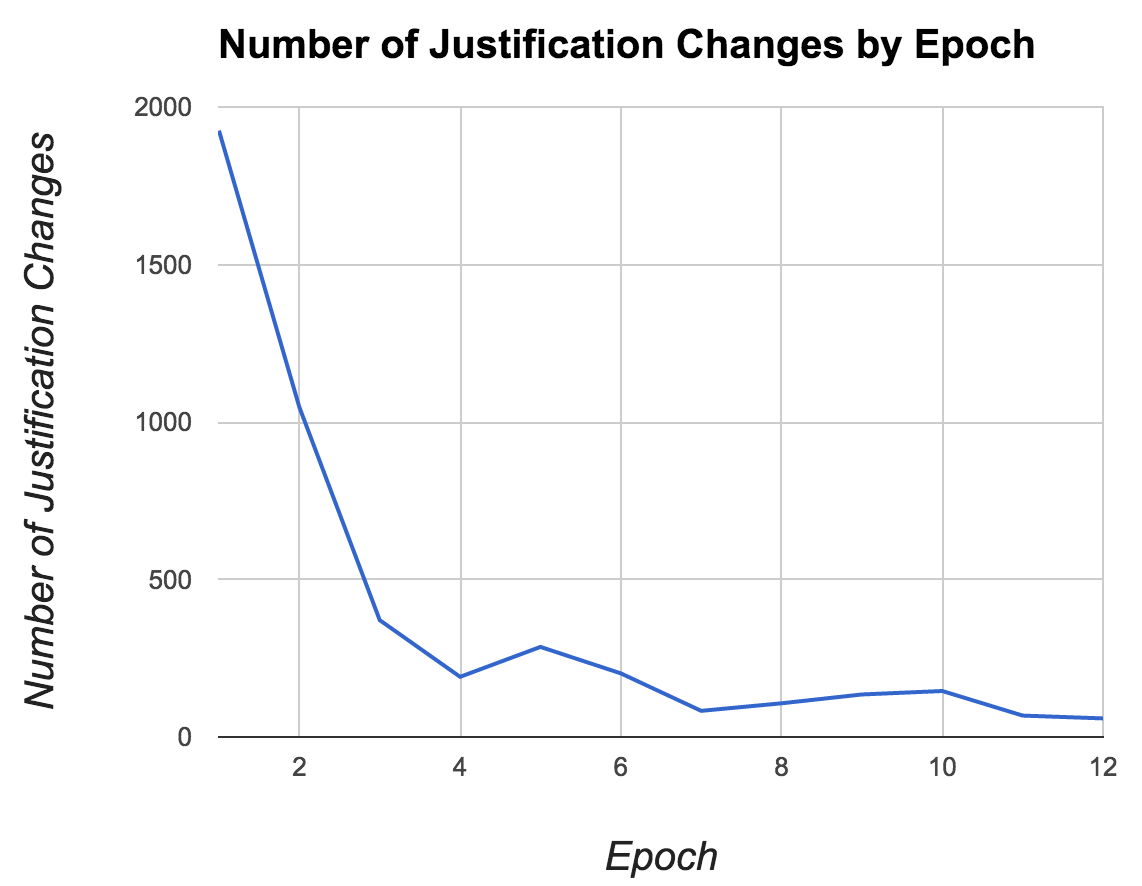
\includegraphics[width=0.7\textwidth]{mainmatter/emnlp2017-qaj/justificationChanges.png}
\caption{Number of questions for which % the IR$^{++}$ + EF + lexDisc + Emb 
our complete model chooses a new justification at each epoch during training.  While this is for a single random seed, we see essentially identical graphs for each random initialization.}
\label{fig:changes}
%space{-5mm}
\end{center}
\end{figure}

%\subsection{Contribution of Jointly Learning to Rank Justifications}
%\begin{flushleft}
%{\bf Contribution of Learning to Rerank Justifications}
%\end{flushleft}
%space{-2mm}
\paragraph{Contribution of Learning to Rerank Justifications:}
The main assertion of this work is that through learning to rank answers and justifications for those answer candidates in an end-to-end manner, we both answer questions correctly and provide justifications as to why the answer is correct.  To confirm that this is the case, we also ran a version of our system that does not re-rank justifications, but uses the top-ranked justification retrieved by IR.  This configuration dropped our performance on test to 48.7\% P@1, a decrease of 4.6\%, and we additionally lose all justification improvements from our system (see Section \ref{sec-emnlp2017:justification_results}), demonstrating that learning this reranking is key to our approach.

Additionally, we tracked the number of times a new justification was chosen by the model as it trained. We found that our system converges to a stable set of justifications during training, shown in Figure \ref{fig:changes}.



\begin{table}[t]
\begin{center}
\begin{tabular}{ll}
\hline
Error Type & Percent \\ 
\hline
Short justification/High lexical overlap  & 53.3\%\\
Complex inference required   & 43.3\% \\
Knowledge Base Noise  & 6.7\% \\
Word order necessary	 & 6.7\% \\
Coverage & 6.7\% \\
Negation	& 3.3\% \\
Other & 6.7\% \\
\end{tabular}

\caption{{ Summary of the findings of the 30 question error analysis.  
Examples of several categories are provided in separate tables. 
Note that a given question may fall into more than one category.}} 
\label{tab:erroranalysis}
\vspace{-5mm}
\end{center}
\end{table}

%\begin{table}[!th]
%\begin{center}
%\begin{footnotesize}
%\hfill
%\begin{tabular}{p{0.8cm}p{6.5cm}p{1cm}}
%\hline
%\multicolumn{2}{l}{Error Type} & Percent \\ 
%\hline
%\multicolumn{2}{l}{\textbf{Shorter justification with lots of lexical overlap}} & 53.3\%\\
%\multicolumn{2}{l}{\textbf{Complex inference required}}  & 43.3\% \\
%\hline
%
%\\
%\hline
%\multicolumn{2}{l}{\textbf{KB Noise}}  & 6.7\% \\
%\hline
%Question: & \multicolumn{2}{p{7.5cm}}{ If an object traveling to the right is acted upon by an unbalanced force from behind it  the object will}	\\
%Correct: & \multicolumn{2}{p{7.5cm}}{speed up }	\\
%Chosen & \multicolumn{2}{p{7.5cm}}{ change direction }	\\
%			& \multicolumn{2}{p{7.5cm}}{\textit{ Unbalanced force: force that acts on an object that will change its direction}}	\\
%%\hline
%\multicolumn{3}{p{8cm}}{The system found a sentence in the knowledge base that "justifies" the correct answer.}	\\
%%
%\\
%\hline
%\multicolumn{2}{l}{\textbf{Word order necessary}}	 & 6.7\% \\
%\hline
%Question: & \multicolumn{2}{p{7.5cm}}{ The acceleration of a small rocket that has just been launched can be quantitatively found by}	\\
%Correct: & \multicolumn{2}{p{7.5cm}}{dividing the force acting upon the rocket by its mass }	\\
%Chosen & \multicolumn{2}{p{7.5cm}}{ dividing the mass of the rocket by the force acting upon it }	\\
%			& \multicolumn{2}{p{7.5cm}}{\textit{ (same for both) acceleration: force divided by mass}}	\\
%%\hline
%\multicolumn{3}{p{8cm}}{The ordering of the answer choice terms was necessary for answering the question.}	\\
%%
%\\
%\hline
%\multicolumn{2}{l}{\textbf{Coverage}} & 6.7\% \\
%\hline
%Question: & \multicolumn{2}{p{7.5cm}}{ Which activity most effectively ensures the proper functioning of osteocytes?}	\\
%Correct: & \multicolumn{2}{p{7.5cm}}{consuming mineral-rich foods}\\
%			& \multicolumn{2}{p{7.5cm}}{\textit{ most lipids consumed from food are in the form of triglycerids}}	\\	
%Chosen & \multicolumn{2}{p{7.5cm}}{increasing the respiratory rate }	\\
%			& \multicolumn{2}{p{7.5cm}}{\textit{ hyperventilation increased respiratory rate}}	\\
%%\hline
%\multicolumn{3}{p{8cm}}{The knowledge base had no coverage for the concept of \emph{osteocyte}, so the system grasped at proverbial straws.}	\\
%%
%\\
%\hline
%\multicolumn{2}{l}{\textbf{Negation}}	& 3.3\% \\
%\hline
%%\multicolumn{3}{l}{Example}	\\
%Question: & \multicolumn{2}{p{7.5cm}}{ Which feature does not form as a result of tectonic plates diverging?}	\\
%Chosen: & \multicolumn{2}{p{7.5cm}}{ rift valley }	\\
%			& \multicolumn{2}{p{7.5cm}}{\textit{ Rift valley: deep valley formed as tectonic plates move apart. }}	\\
%\multicolumn{3}{p{8cm}}{Note that the justification actually shows that the chosen answer is incorrect, rather than justifying it.  This is the expected behavior for the system for these negated questions as we don't handle them differently.}	\\
%%
%\\
%\hline
%\multicolumn{2}{l}{\textbf{Other}} & 6.7\% \\
%\end{tabular}
%\hfill
%\end{footnotesize}
%\caption{{\footnotesize Summary of the findings of the 30 question error analysis.  Note that a given question may fall into more than one category.}} 
%\label{tab:erroranalysis}
%\end{center}
%\end{table}

\begin{table}[t]
\begin{center}
\begin{tabular}{p{2cm}p{12cm}}
\hline
Type: & \textbf{Short justification/High lexical overlap}\\
\hline
Question: & The length of time between night and day on Earth varies throughout the year. This time variance is explained primarily by $\rule{1cm}{0.15mm}$. \\
\\
Correct: & Earth 's angle of tilt \\
			 & \textit{ ... the days are very short in the winter because the sun's rays hit the earth at an extreme angle ... due to the tilt of the earth's axis. } \\
\\
Chosen: &  Earth 's distance from the Sun \\
			& \textit{ Is light year time or distance? Distance}	\\
\end{tabular}
\caption{{ Example of the system preferring a justification for which all the terms were found in either the question or answer candidate, while the justification for the correct answer contained additional information necessary to fully explain the answer. 
(Justifications shown in italics)
}} 
\label{tab:ex_lex_overlap}
\end{center}
\end{table}

\subsection{Error Analysis}
\label{sec-emnlp2017:erroranalysis}

To better understand the limitations of our current system, we performed an error analysis of 30 incorrectly answered questions.  
We examined the top 5 justifications returned for both the correct and chosen answers.  
Notably, 50\% of the questions analyzed had one or more good justifications in the top 5 returned by our system, but for a variety of reasons, summarized in Table \ref{tab:erroranalysis}, the system incorrectly ranked another justification higher.  

The table shows that the most common form of error was the system's apparent preference for short justifications with a large degree of lexical overlap with the question and answer choice itself, shown by the example in Table \ref{tab:ex_lex_overlap}.  The effect was magnified when the correct answer required more explanation to connect the question to the answer.  
This suggests that the system has learned that generally many unmatched words are indicative of an incorrect answer.  While this may typically be true, extending the system to be able to prefer the \emph{opposite} with certain types of questions would potentially help with these errors.  

\begin{table}[!th]
\begin{center}
\begin{tabular}{p{2cm}p{12cm}}
\hline
Type: & \textbf{Complex inference required}\\
\hline
Question: & Mr. Harris mows his lawn twice each month. He claims that it is better to leave the clippings on the ground. Which long term effect will this most likely have on his lawn? \\
\\
Correct: &  It will provide the lawn with needed nutrients. \\	
\end{tabular}
\caption{{ Example of a question for which complex inference is required.  In order to answer the question, you would need to assemble the event chain: cut grass left on the ground $\rightarrow$ grass decomposes $\rightarrow$ decomposed material provides nutrients.}} 
\label{tab:ex_complex_inf}
\end{center}
\end{table}

The second largest source of errors came from questions requiring complex inference (causal, process, quantitative, or model-based  reasoning) as with the question shown in Table \ref{tab:ex_complex_inf}.  This demonstrates not only the difficulty of the question set but also the need for systems that can robustly handle a variety of question types and their corresponding information needs.  


%The second largest source of errors came from questions requiring complex inference (causal, process, quantitative, or model-based  reasoning) as with the question:%.  For example, to answer the question:
 %\begin{quote}
%\begin{addmargin}[1em]{2em}% 1em left, 2em right 
% \begin{footnotesize}
%  \textit{Q: Mr. Harris mows his lawn ...[and leaves] the clippings on the ground. Which long term effect will this most likely have on his lawn? \\
%  A: It will provide the lawn with needed nutrients.}
% \end{footnotesize}
%%\end{quote}
%\end{addmargin}
%To answer this, you would need to link together: \textit{cut grass left on the ground $\rightarrow$ grass decomposes $\rightarrow$ decomposed material provides nutrients}. 
%These questions constitute a large portion of our errors,  
%is a large set of questions that our system is not particularly designed to handle, 
%demonstrating not only the difficulty of the question set but also the need for systems that can robustly handle a variety of question types and their corresponding information needs.  

\begin{table}[t]
\begin{center}
%\begin{footnotesize}
\begin{tabular}{p{2cm}p{12cm}}
\hline
Type: & \textbf{Knowledge base noise}\\
\hline
Question: & If an object traveling to the right is acted upon by an unbalanced force from behind it the object will $\rule{1cm}{0.15mm}$.\\
\\
Correct: & speed up\\
			%& \textit{Change of speed: an object accelerates if it speeds up and decelerates when it slows down}	\\	
\\
Chosen & change direction 	\\
			& \textit{ Unbalanced force: force that acts on an object that will change its direction}	\\
\end{tabular}
%\end{footnotesize}
\caption{{ Example of a question for which knowledge base noise (here, in the form of over-generalization) was an issue.}} 
\label{tab:ex_noise}
\end{center}
\end{table}


Aside from these primary sources of error, there were some smaller trends:  
7\% of the incorrectly chosen answers actually had justifications which ``validated'' them due to noise in the knowledge base (e.g., the example shown in Table \ref{tab:ex_noise}), 7\% required word-order to answer (e.g., \emph{mass divided by acceleration} vs. \emph{acceleration divided by mass}), another 7\% of questions suffered from lack of coverage of the question concept in the knowledge base,
%(see example in Table \ref{tab:ex_coverage}), 
 and 3\% failed to appropriately handle negation (i.e., questions of the format \emph{Which of the following are NOT ...}). 

%
%
%% bs: no room: - Negative results?


%\begin{table}[t]
%\begin{center}
%\begin{footnotesize}
%\begin{tabular}{p{1cm}p{6cm}}
%\hline
%Type: & \textbf{Coverage}\\
%\hline
%Question: & Which activity most effectively ensures the proper functioning of osteocytes? \\
%Correct: & consuming mineral-rich foods\\
%			& \textit{ most lipids consumed from food are in the form of triglycerids}	\\	
%Chosen & increasing the respiratory rate 	\\
%			& \textit{ hyperventilation increased respiratory rate}	\\
%\end{tabular}
%\hfill
%\end{footnotesize}
%\caption{{\footnotesize Example of a question for which coverage was an issue.  The KB had no coverage for the concept of \emph{osteocyte}.}} % , so the system grasped at proverbial straws.}} 
%\label{tab:ex_coverage}
%\end{center}
%\end{table}

 

%%\begin{table}[!th]
%\begin{center}
%\begin{footnotesize}
%\hfill
%\begin{tabular}{ll}
%\hline
%Error Type & Percent \\ 
%\hline
%Short justification/High lexical overlap  & 53.3\%\\
%Complex inference required   & 43.3\% \\
%Knowledge Base Noise  & 6.7\% \\
%Word order necessary	 & 6.7\% \\
%Coverage & 6.7\% \\
%Negation	& 3.3\% \\
%Other & 6.7\% \\
%\end{tabular}
%\end{footnotesize}
%\caption{{\footnotesize Summary of the findings of the 30 question error analysis.  
%%Examples of several categories provided in separate tables. 
%Note that a given question may fall into more than one category.}} 
%\label{tab:erroranalysis}
%\vspace{-5mm}
%\end{center}
%\end{table}


%\begin{table}[t]
%\begin{center}
%\begin{footnotesize}
%\begin{tabular}{p{1cm}p{6cm}}
%\hline
%Type: & \textbf{Short justification/High lexical overlap}\\
%\hline
%Question: & The length of time between night and day on Earth varies throughout the year. This time variance is explained primarily by $\rule{1cm}{0.15mm}$. \\
%Correct: & Earth 's angle of tilt \\
%			 & \textit{ ... the days are very short in the winter because the sun's rays hit the earth at an extreme angle ... due to the tilt of the earth's axis. } \\
%Chosen: &  Earth 's distance from the Sun \\
%			& \textit{ Is light year time or distance? Distance}	\\
%\end{tabular}
%\hfill
%\end{footnotesize}
%\caption{{\footnotesize Example of the system preferring a justification for which all the terms were found in either the question or answer candidate. (Justifications shown in italics)
%}} 
%\label{tab:ex_lex_overlap}
%\vspace{-5mm}
%\end{center}
%\end{table}

\subsection{Error Analysis}
\label{sec-emnlp2017:erroranalysis}

We performed an error analysis of 30 incorrectly answered questions, %summarized in Table \ref{tab:erroranalysis},
  examining the top 5 justifications returned for both the correct and chosen answers of each.    
%Among the questions analyzed we found some interesting trends.   
Notably, 50\% of the questions had one or more \emph{Good} justifications. %, but the system incorrectly ranked another answer's justification higher.  
The most common form of error (53.3\%) was due to the system's preference for short justifications with a large degree of lexical overlap with the question and answer choice, %, particularly when the correct answer required more "explanation" to connect the question to the answer.  
% shown by the example in Table \ref{tab:ex_lex_overlap}.  
 %This effect was magnified when the correct answer required more "explanation" to connect the question to the answer.  
suggesting the system has learned that generally many unmatched words are indicative of an incorrect answer.  %While this may typically be true, extending the system to be able to prefer the \emph{opposite} with certain types of questions would potentially help with these errors.  
The second largest source of errors (43.3\%) came from questions requiring complex inference (causal, process, quantitative, or model-based reasoning), demonstrating the difficulty of the question set and the need for systems that can robustly handle a variety of question types.
Aside from these main groups, there were some smaller trends including KB noise, and our system's lack of using word order and recognizing negation.\footnote{A much more detailed error analysis is available, and if this paper is accepted will be included.}
 
% as with the question:%.  For example, to answer the question:
 %\begin{quote}
%\begin{addmargin}[1em]{2em}% 1em left, 2em right 
% \begin{footnotesize}
%  \textit{Q: Mr. Harris mows his lawn ...[and leaves] the clippings on the ground. Which long term effect will this most likely have on his lawn? \\
%  A: It will provide the lawn with needed nutrients.}
% \end{footnotesize}
%%\end{quote}
%\end{addmargin}
%To answer this, you would need to link together: \textit{cut grass left on the ground $\rightarrow$ grass decomposes $\rightarrow$ decomposed material provides nutrients}. 
%These questions constitute a large portion of our errors,   demonstrating not only the difficulty of the question set but also the need for systems that can robustly handle a variety of question types and their corresponding information needs.  

%Aside from these main groups, there were some smaller trends including:  
%7\% of the incorrectly chosen answers actually had justifications which "validated" them due to KB noise, 7\% required word-order to answer (e.g., \emph{X divided by Y} vs. \emph{Y divided by X}), %another 7\% of questions suffered from lack of coverage of the question concept in the knowledge base,
%%(see example in Table \ref{tab:ex_coverage}), 
% and 3\% failed to appropriately handle negation (i.e., questions of the format \emph{Which of the following are NOT ...}). 


% bs: no room: - Negative results?


%\begin{table}[t]
%\begin{center}
%\begin{footnotesize}
%\begin{tabular}{p{1cm}p{6cm}}
%\hline
%Type: & \textbf{Coverage}\\
%\hline
%Question: & Which activity most effectively ensures the proper functioning of osteocytes? \\
%Correct: & consuming mineral-rich foods\\
%			& \textit{ most lipids consumed from food are in the form of triglycerids}	\\	
%Chosen & increasing the respiratory rate 	\\
%			& \textit{ hyperventilation increased respiratory rate}	\\
%\end{tabular}
%\hfill
%\end{footnotesize}
%\caption{{\footnotesize Example of a question for which coverage was an issue.  The KB had no coverage for the concept of \emph{osteocyte}.}} % , so the system grasped at proverbial straws.}} 
%\label{tab:ex_coverage}
%\end{center}
%\end{table}


%\begin{table}[!th]
%\begin{center}
%\begin{footnotesize}
%\begin{tabular}{p{1cm}p{6cm}}
%\hline
%Type: & \textbf{Complex inference required}\\
%\hline
%Question: & Mr. Harris mows his lawn twice each month. He claims that it is better to leave the clippings on the ground. Which long term effect will this most likely have on his lawn? \\
%Correct: &  It will provide the lawn with needed nutrients. 	\\
%\end{tabular}
%\hfill
%\end{footnotesize}
%\caption{{\footnotesize Example of a question for which complex inference is required.  In order to answer the question, you would need to assemble the following chain of events: cut grass left on the ground $\rightarrow$ grass decomposes $\rightarrow$ decomposed material provides nutrients.}} 
%\label{tab:ex_complex_inf}
%\end{center}
%\end{table}


\section{Conclusion}
\label{sec-emnlp2017:conclusions}

Here we propose an end-to-end question answering (QA) model that learns to correctly answer questions as well as provide compelling, human-readable justifications for its answers,  despite not having access to labels for justification quality.  We do this by using the question answering task as a form of distant supervision for learning  justification re-ranking.  Similar in nature to the model proposed in Chapter \ref{chapter:cl2017}, we differ primarily in the shallower representation of our knowledge base texts (sentences versus graphlets) and the lack of aggregation in forming justifications.  These differences render this model more versatile -- they allow us to utilize larger corpora and consequently handle more challenging question sets that require more diverse background information to answer.   We show that our accuracy and justification quality are significantly better than a strong IR baseline, while maintaining near state-of-the-art performance for the answer selection task as well.  That is, without unduly sacrificing accuracy, with this approach we are able to provide explanations that complete the inference needed to connect questions and their answers.
%for selected answers that complete the inference to connect them to the corresponding questions.

Of the different types of features included in the model, we found that the explicit lexical overlap features were the most useful, and that the discourse and word embedding-based features each provided only a slight performance boost.  For the embedding-based features, this could be due to the limited amount of training data (often, neural networks that successfully learn feature representations operate over orders of magnitude more data than what we have available here).  Indeed, we found that when we attempted to update the word embeddings we ran into issues with  overfitting.  

Regarding the discourse features, with this approach we do not particularly address the different information needs of distinct question types (see \ref{sec:intro_emnlp2016}; cf., Chapter \ref{chapter:emnlp2016}), but intuitively different discourse relations may be more or less relevant to to each of them.  For example, a \textit{cause} relation may be more relevant to a causal question than it is to a definitional question.  Since our approach here does not allow for specialization of the model to different question types, this could be the reason for the underperformance of this discourse-based feature group.
%With this approach we do not particularly address the different information needs of distinct question types (see \ref{sec:intro_emnlp2016}; cf., Chapter \ref{chapter:emnlp2016}).  
Also, as discussed in the error analysis in Section \ref{sec-emnlp2017:erroranalysis}, of the incorrectly answered questions analyzed, 43.3\% required a form of complex inference such as \textit{causal} or \textit{quantitative} reasoning.  We hypothesize that by attempting to apply the same model to \textit{all} question types, we aren't able to specialize enough to handle these more complex information needs.   
While this framework can be extended to allow the model to learn different priorities for justification selection given different question information needs (perhaps similarly to the domain adaptation-based method that is used in Section \ref{sec-cl2017:characterizing}), we leave that extension to future work.  

Additionally, not performing aggregation to construct justifications constitutes a trade-off -- the approach is more lightweight (i.e., faster to run, and able to handle larger corpora within a given resource limit), but it becomes less likely that there exists a \textit{complete} justification for more complicated questions.  Likely there is a way to better balance the two -- perhaps by performing only selected aggregation during pre-processing, for topics that are more likely to need more than a single sentence to express.  Alternatively, perhaps reinforcement learning could be used to learn \textit{when} to add another sentence to an existing candidate justification for a given question and answer.  Again, we leave this exploration to future work.
%\FloatBarrier


%\section*{Acknowledgments}

%\bibliography{refs}
%\bibliographystyle{emnlp_natbib}
%
%\end{document}
